% #############################################################################
% This is Chapter 6
% !TEX root = ../main.tex
% #############################################################################
% Change the Name of the Chapter i the following line
\fancychapter{User Studies}
%\cleardoublepage
% The following line allows to ref this chapter
\label{chap:UserStudies}
To evaluate the developed Trust Model we conducted a user study using the Quick Numbers scenario  (Figure \ref{fig:ParticipantQuickNumbers}) previously described in Chapter \ref{chap:Scenario}, and \ac{EMYS} (Figure \ref{fig:EMYS}) as the robot to embody the virtual agent. Additionally, the user study was also executed in conjunction with Henriques to test his own Rapport model. The study was performed in a between subjects design, focusing on checking if Trust would increase between conditions where the model's Action Suggestion component is either active or inactive. Trust is measured through a questionnaire, later described in Section \ref{subsec:Questionnaire} the Investment scenario value.



\begin{figure}[h]
    \centering
    \begin{minipage}[b]{.60\textwidth}
        \centering
        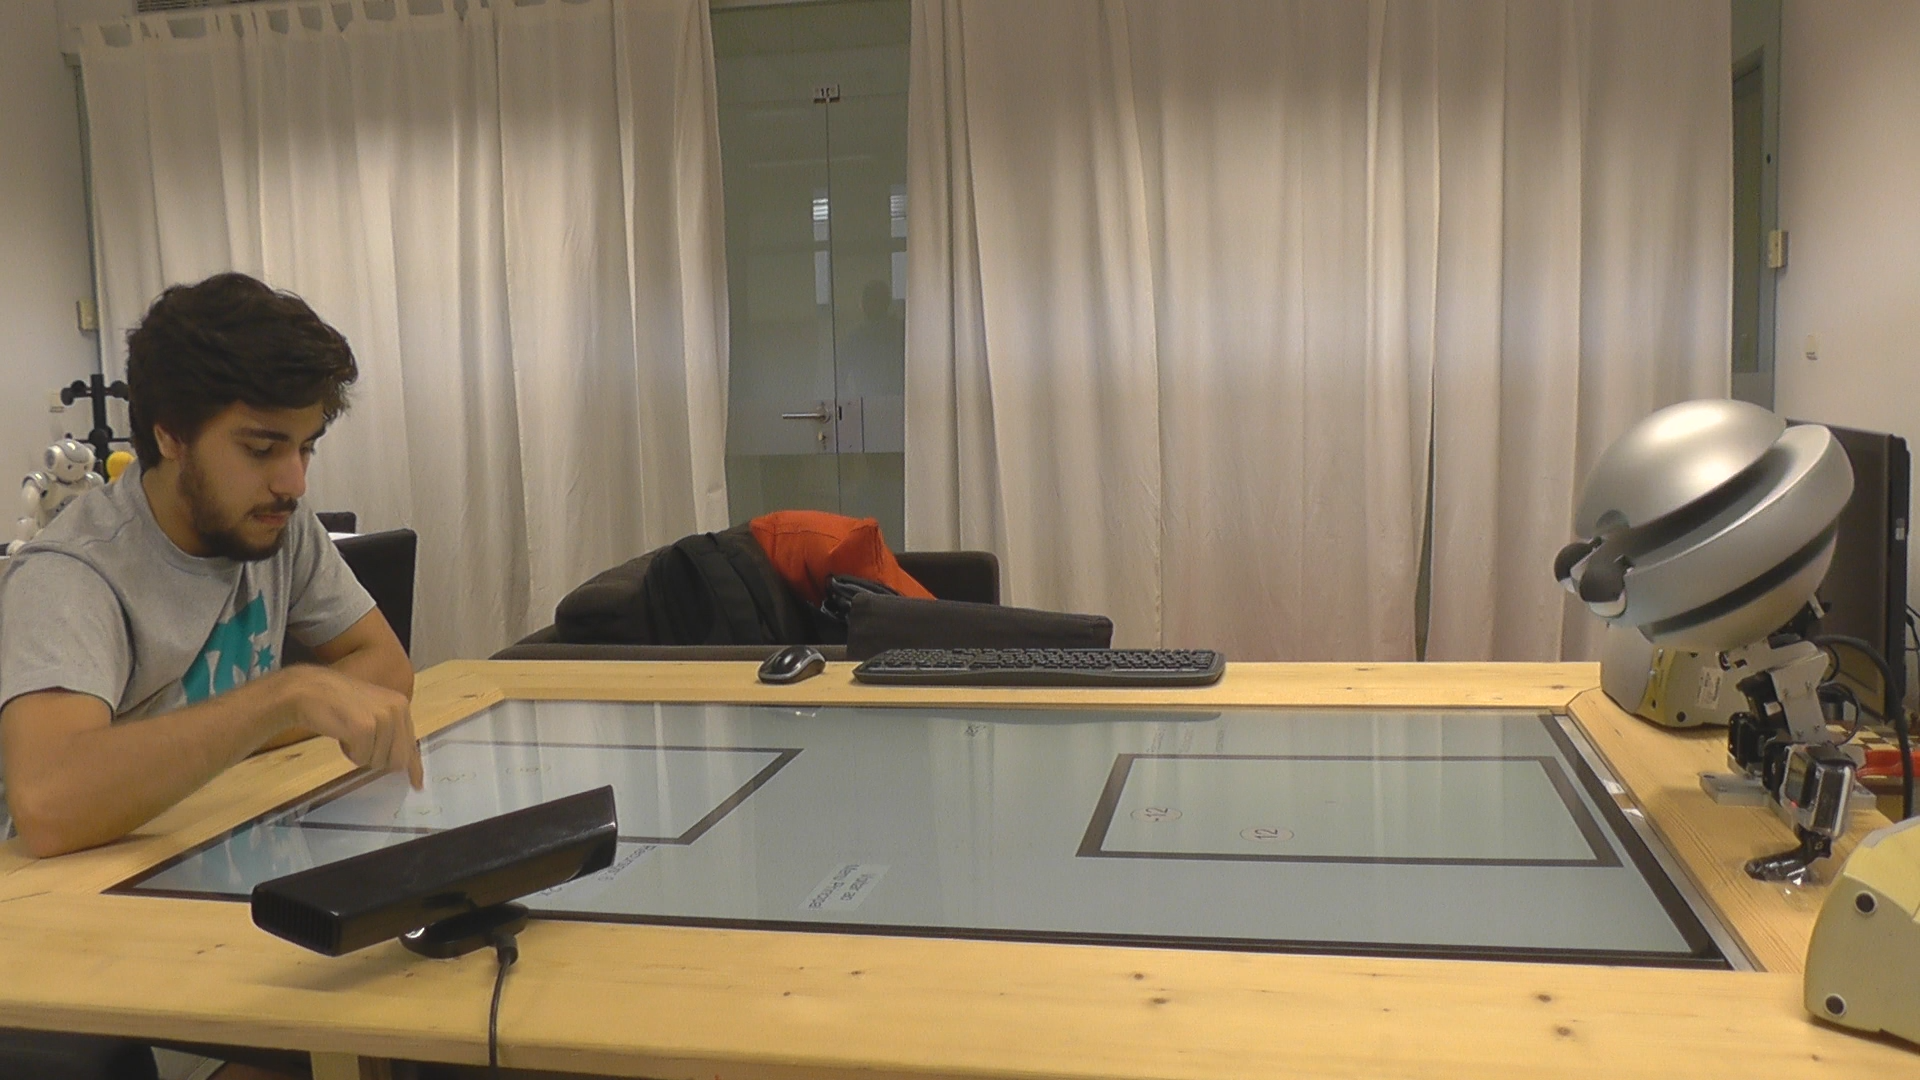
\includegraphics[width=\textwidth]{figures/ScenarioScreenShot.png}
        \caption{Participant playing with \ac{EMYS} in the Quick Numbers scenario}
        \label{fig:ParticipantQuickNumbers}
    \end{minipage}
    \hfill
    \begin{minipage}[b]{.30\textwidth}
        \centering
        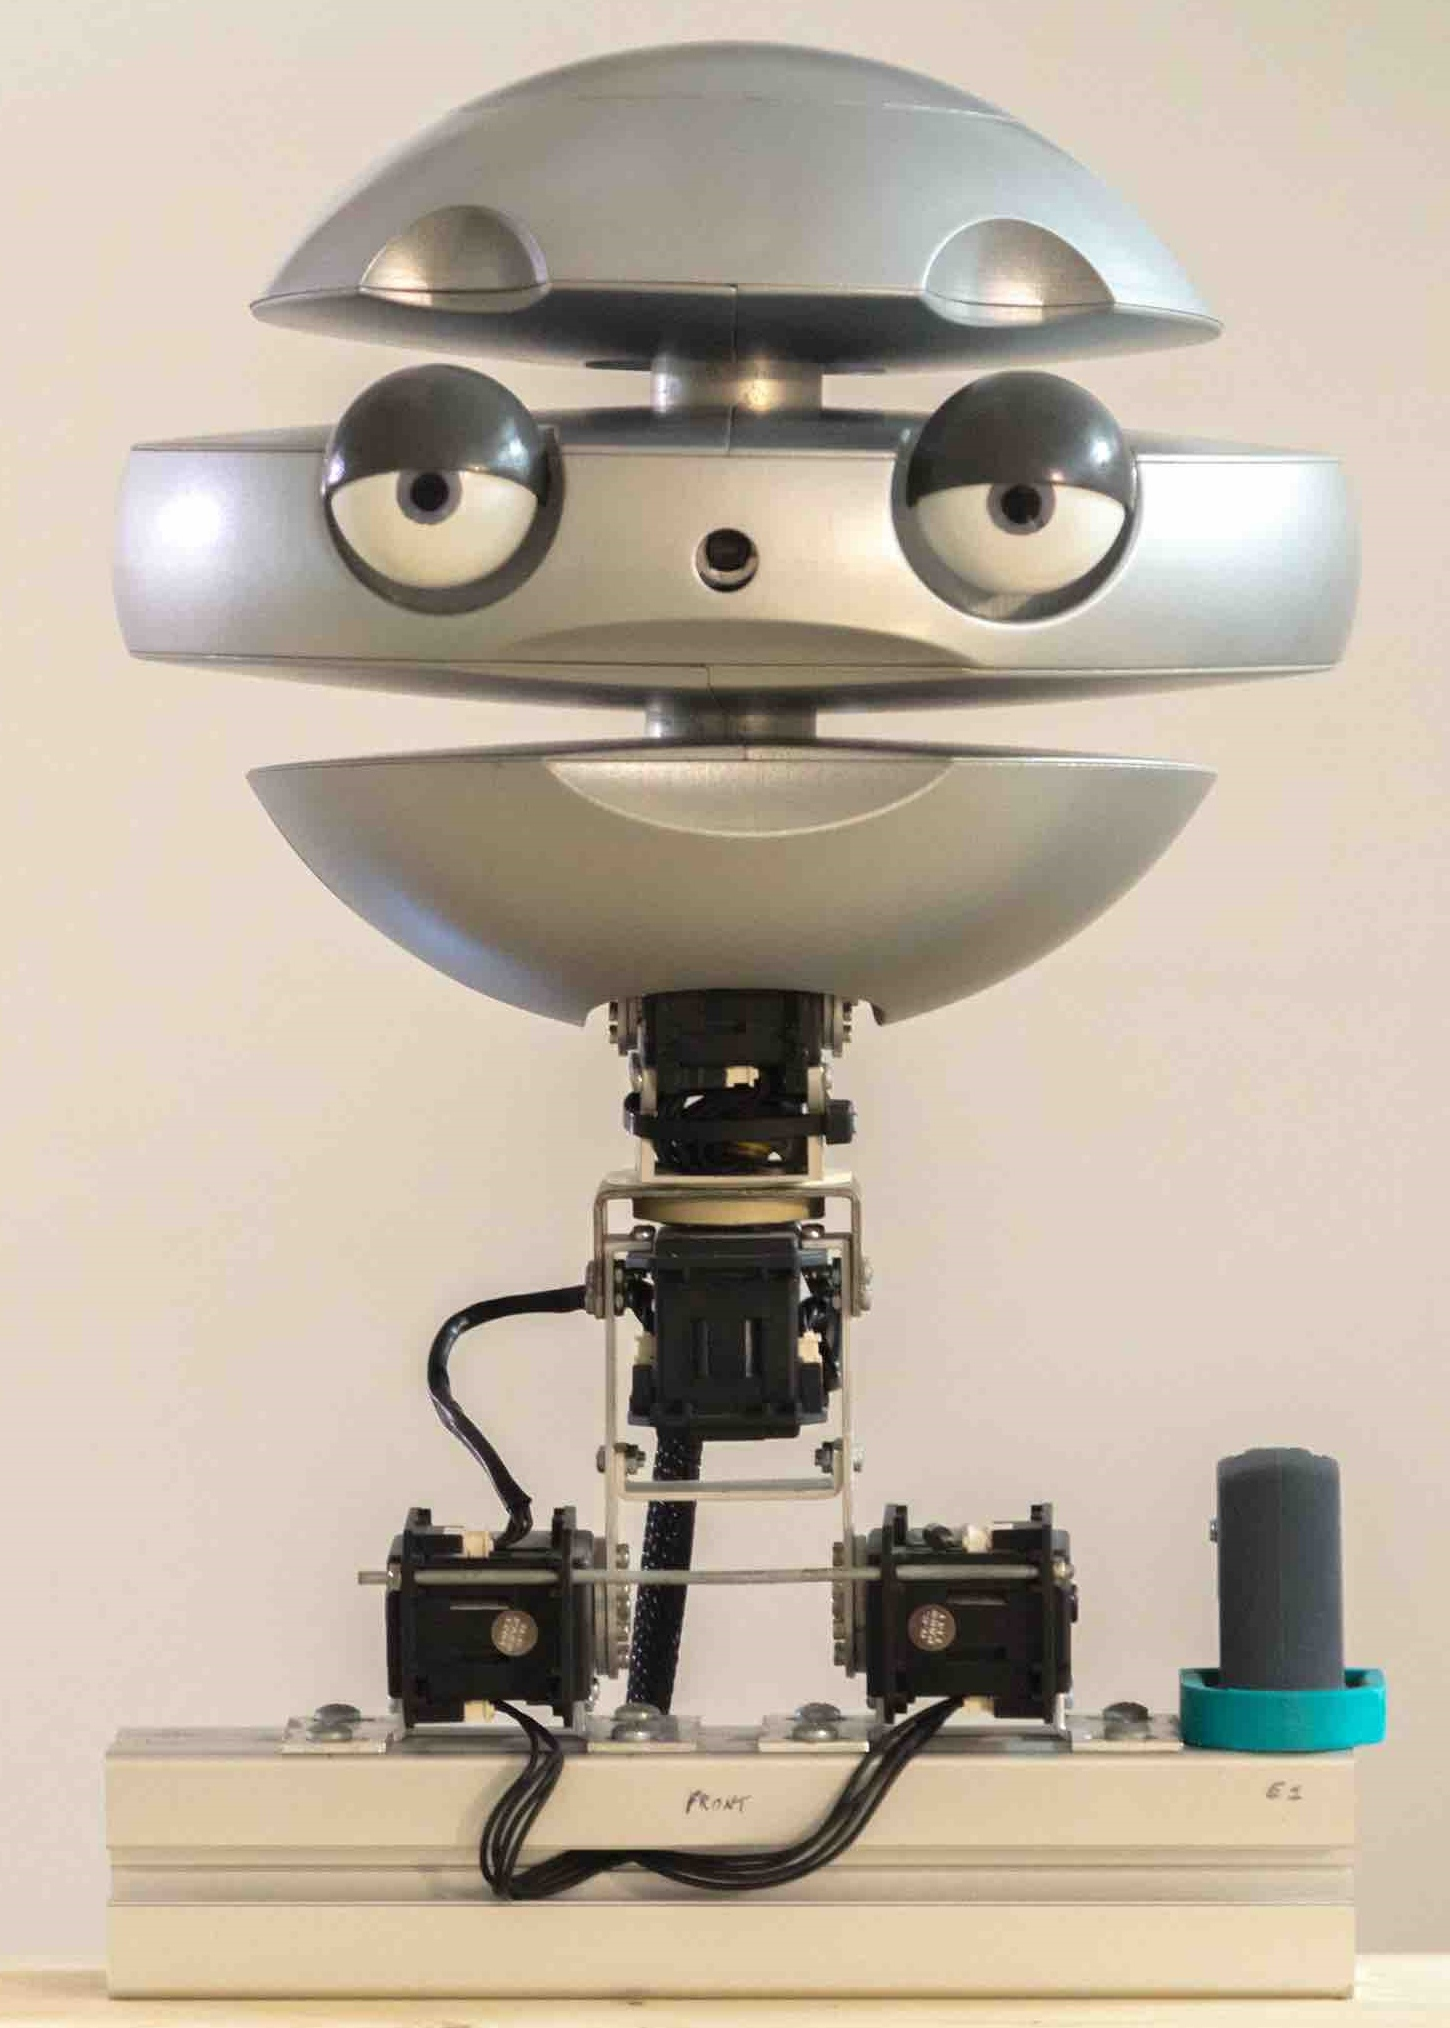
\includegraphics[width=\textwidth]{figures/emys.jpg}
        \caption{\ac{EMYS} Robot}
        \label{fig:EMYS}
    \end{minipage}
\end{figure}

\section{Agent Architecture}
The agent we used to serve as a host to the Trust Model was built using Henriques' Rapport Controller \cite{Henriques2016}, a computational framework developed to create human agent interactions and transmit them to the various components that control the agent embodiment. This version of the framework is built upon \ac{SERA}'s ecosystem \cite{Ribeiro2003}, an architectural model that gathers and connects a series of tools to control a robotic embodiment, namely:

\begin{itemize}
    \item \textbf{Thalamus}: A networking module that enables the exchange of actions and perceptions between the various agent's modules. All communication coming from the controller to the robot actuators and scenario sensors come through this module;
    \item \textbf{Skene}: A behaviour planner that translates high-level intentions to actions. For the purpose of the Rapport Controller the main use of Skene is to perform animation planning, lip-syncing and handling gaze. Additionally, it provides simple way to input these intentions, through a simple markup language.
    \item \textbf{Nutty Tracks}: An animation engine that performs the animations of the embodied agent;
    \item \textbf{Speech Server}: A simple \ac{TTS} server to perform utterances.
\end{itemize}
              
The Rapport Controller uses a plug-in architecture, and for the purpose of this thesis we will focus on describing plug-ins made for the Controller to represent the Trust Model and the Scenario.
                                                                    
\subsection{Trust Model Implementation}
The Trust Model was implemented as a plug-in to the Rapport Controller. Although 


\section{Methodology and Procedures}
The study was conducted with a between subject design with the following conditions:
\begin{itemize}
    \item \textbf{Condition B}: a baseline condition, where the Action Suggestion component is not active. The data gathered in this condition will serve as the basis to which we compare our results;
    \item \textbf{Condition T}: the condition where Action Suggestion is active, serving as the main results condition.
    \item \textbf{Condition R}: a condition using Henriques' Rapport Model;
    \item \textbf{Condition T+R}: a condition using both ours Action Suggestion component and Henriques' Rapport Model.
\end{itemize}

The conditions R and T+R go out of the scope of this thesis and will not be addressed in this document.

The user study sessions were individual and performed in an closed room accompanied just by the researcher, and lasted between 20 and 30 minutes. The sessions followed the stages as described in Section \ref{sub:stages}. Additionally the participants answered a questionnaire, described in Section \ref{subsec:Questionnaire}, which is divided in 3 sections, to be filled in different stages of the scenario,

\subsection{Questionnaire}
\label{subsec:Questionnaire}
The questionnaire we requested the participants to answer is a conjunction of 5 different parts:

\begin{itemize}
    \item 
\end{itemize}

\section{Scenario Parametrization}



\section{Results}
